In the second iteration of the cell board, control of the cell board was implemented in software instead of controlling via hardware.
This implementation was done to allow for more flexibility in the control of the cells to allow for changing cell characteristics without the need for hardware changes.
The software in this iteration has only the bare framework for individual cell control.
The hardware is controlled digitally through the use of digital potentiometers. The resistance of the digital potentiometers correspond linearly to the voltage and current of the cell.

\subsubsection{Software Architecture}
If there were to be a user interface, each cell would be an object of the CellEmulator class and can be controlled individually. Fig. \ref{fig:classDiagram} lists the attributes and methods of the CellEmulator class. The attributes are stored privately and can only be accessed through the methods. The methods are the only way to interact with the cell. 
\FloatBarrier
\begin{figure}[ht!]
    \centering
    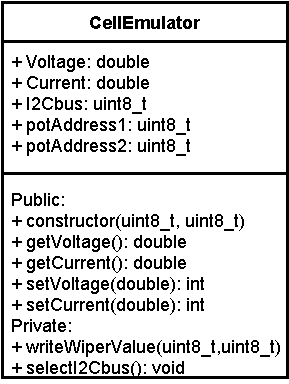
\includegraphics[scale=0.7]{classDiagram.pdf}
    \caption{Class definition diagram}
    \label{fig:classDiagram}
\end{figure}
\FloatBarrier
The methods are listed in the bottom cell of Fig. \ref{fig:classDiagram} and the flowcharts can be found in Appendix \ref{sec:software_flowcharts}. The getVoltage and getCurrent methods simply return the internally stored voltage and current of the cell respectively. The setVoltage method takes a voltage value and converts it to the correct wiper value (range 0 to 255). It then calls the writeWiperValue method to write the wiper value to the digital potentiometer. The setCurrent method does the same thing as the setVoltage method, but for current.

The private methods writeWiperValue and SelectI2Cbus are both used to write the correct value to the correct digital potentiometer. The writeWiperValue method writes the value to the digital potentiometer. The SelectI2Cbus method selects the correct I2C bus to write to. 
This is necessary because the potentiometers for the current sink have 3 address bits (which are set in hardware) resulting in 8 unique addresses, and the potentiometers for the voltage source have 2 address bits resulting in 4 unique addresses. The constant address of the 2 types of potentiometers are different. Therefore, there can be 4 cells on a single I2C bus, resulting in 4 I2C busses for 14 cells. 
